%\subsection{Omówienie wyników}
%\label{subsec:omowienie-wynikow}

W trakcie działania programu przeprowadzono $210$ gier.
System lichess-bot został skonfigurowany w taki sposób, aby akceptować wyzwania jedynie dla gier typu \texttt{bullet} oraz \texttt{blitz}, oraz dla oponentów z rankingiem odstającym o $\pm300$ od rankingu silnika.

W momencie zakończenia prac nad silnikiem osiągnął on ranking $1629$ ELO dla gier typu \texttt{bullet} oraz $1617$ ELO dla gier typu \texttt{blitz}.

\begin{figure}[ht]
    \centering
    \begin{tabular}{@{}ll@{}}
        a) & b) \\
        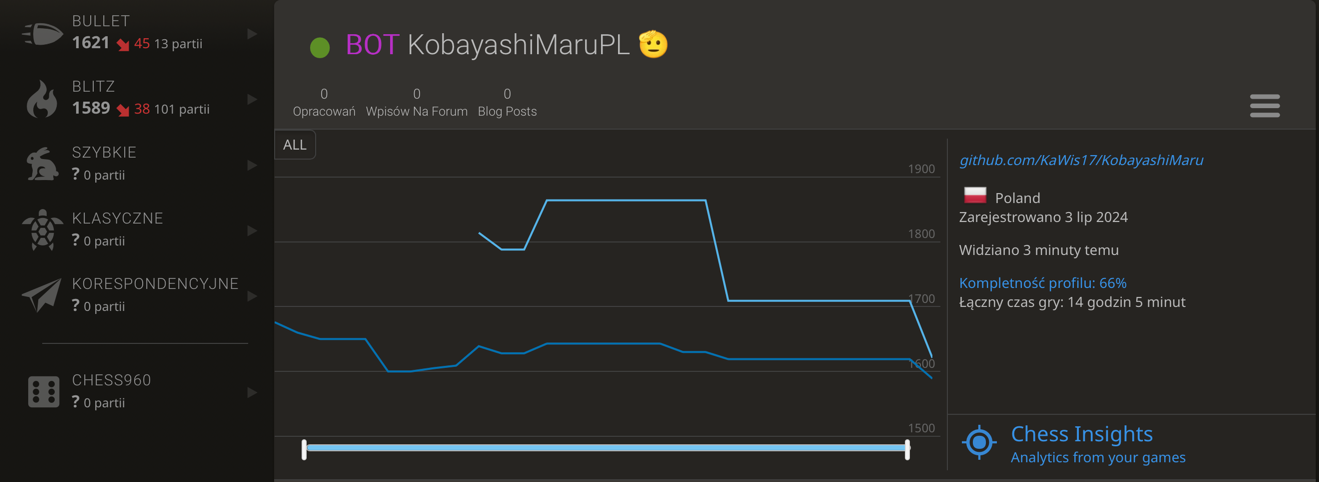
\includegraphics[width=0.45\textwidth]{rozdzialy/rozdzial03/2_porownanie-z-innymi-silnikami/rysunki/lichess-ranking}
        &
        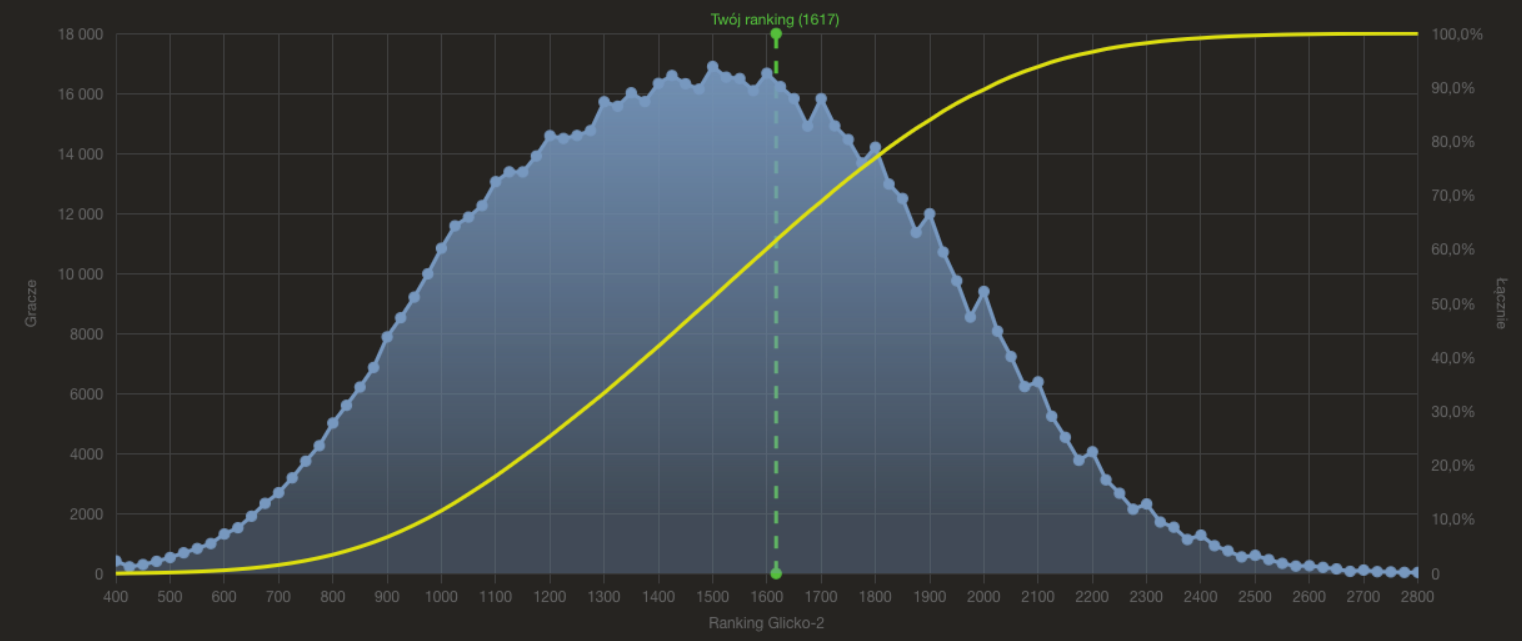
\includegraphics[width=0.5\textwidth]{rozdzialy/rozdzial03/2_porownanie-z-innymi-silnikami/rysunki/lichess-rozklad}
    \end{tabular}
    \caption{Platforma lichess: a) ranking na platformie, b) rozkład rankingów}
    \label{fig: rankig_lichess}

\end{figure}

Platforma Lichess zapewnia również dostęp do narzędzi umożliwiających bardziej szczegółową analizę gier.
Do ich stworzenia wykorzystywany jest jeden z najsilniejszych silników szachowych – Stockfish.
Poniżej przedstawiono niektóre z dostępnych statystyk dla~gier~\texttt{blitz}, wszystkie są wartościami średnimi:
\begin{enumerate}
    \item \textbf{Dokładność gry} – $84.6$\%
    \item \textbf{Ruchów na grę} – $43.41$
    \item \textbf{Gier wygranych} – $41.1$\%
    \item \textbf{Czas ruchu} – $5.65$ sekundy
    \item \textbf{Gier zremisowanych} – $16.9$\%
    \item \textbf{Ranking przeciwnika} – $1\,625.85$ELO
    \item \textbf{Strata względem ruchu optymalnego} – $45.29$ ACPL

\end{enumerate}

Średnia Strata w Centypionach (ang. \emph{Average Centipawn Loss}, w skrócie ACPL) jest miarą oceniającą jakość ruchów gracza.
Wartość ta jest obliczana jako średnia różnica (w setnych częściach wagi piona) pomiędzy ruchem wykonanym przez gracza a ruchem optymalnym \cite*{acpl}.
ACPL na poziomie $0$ oznaczałaby grę idealną, ACPL na poziomie $100$ oznaczaby średnią stratę na~ruch o wartości jednego pionka.
Dla człowieka wartość ACPL równa $20$ jest grą niemal idealną, na~poziomie mistrzowskim \cite*{acpl-2}.

